
\section{Setting up end devices}
Unikernels, similar to traditional OS's can be booted directly from BIOS to hardware. Nevertheless, this is not flexible enough for cloud computing standarts, so hypervisors are used for on demand provisioning of unikernels. For proof of concept development, many different end device configurations were used. There are two different usage scenarios in mind when configuring devices. First one is hypervisor enabled unikernel runtime and the other one is with IoT.

For hypervisor enabled runtime, a laptop was used. Installing a hypervisor on conventional virtual machines in the cloud was not possible because it breaks internal networking and makes it impossible to access machines from outside. Although it would be possible for different cloud providers, it's not a good testing environment as accessing to BIOS of a cloud provided virtual machine is not possible on LRZ.

The mentioned laptop has Debian as the host operating system and Xen was installed through Debian with administrative priviledges to access BIOS. After Xen is installed, when laptop is booted up, user can select to start debian with Xen enabled. It's the same interface that a user sees when dual boots e.g. Windows or Linux. Starting with Xen gives xen daemon access to manipulate hardware. Because a linux system is installed on the computer that communicates with the hypervisor, it's a straightforward process to write Kubernetes clients. That laptop is connected to Kubernetes cluster through a valid kubeconfig file. Figure \ref{fig:hypervisor} shows the final overview of the setup. The virtual-kubelet runs on debian and communicates with Xen trough xen-cli, \textbf{xl}. Two additional linux VM's are traditional Kubernetes nodes connected with kubelet and they are running on the LRZ cloud.

For further testing, a VM with docker daemon was created. This VM does not have a kubelet and runs only virtual-kubelet to communicate with the kubernetes cluster. It still runs docker containers. The provider for that case was called \textit{docker}. It was just for exercising the virtual-kubelet API and is not part of the final setup.

For IoT devices, Raspberry Pi 3 was used. Raspberry Pi uses ARM processor and AMD64 hypervisors can't be ported easily. There is also not too much motivation for it, because Raspberry Pi is not a powerful end-device and not many virtualisation can be done on it. Despite that, there are projects for lightweight virtualisation on Raspberry Pi. For more powerful end devices though, there are hypervisor projects but they are out of scope for this thesis.

To experiment more with unikernel ecosystem, solo5 was installed alongside Xen to the aforementioned laptop. Solo5 can be built on top of Qemu or KVM and it markets itself as a unikernel specific runtime. To test Solo5, Qemu was installed because the hardware didn't allow KVM virtualisation.

Another enviroment is docker containers running virtual-kubelet. They are built on top Ubuntu base image and unikernels can run on them. They are being used to simulate hundreds of IoT machines, since both docker and Raspberry Pis lack hypervisor technology.

When configuring end devices for hypervisors, a network interface for unikernels should be set. If a unikernel application is using networking, the network interface should be given to the boot up command to make the local DHCP give it an IP.


\begin{figure}[htpb]
  
    \centering
    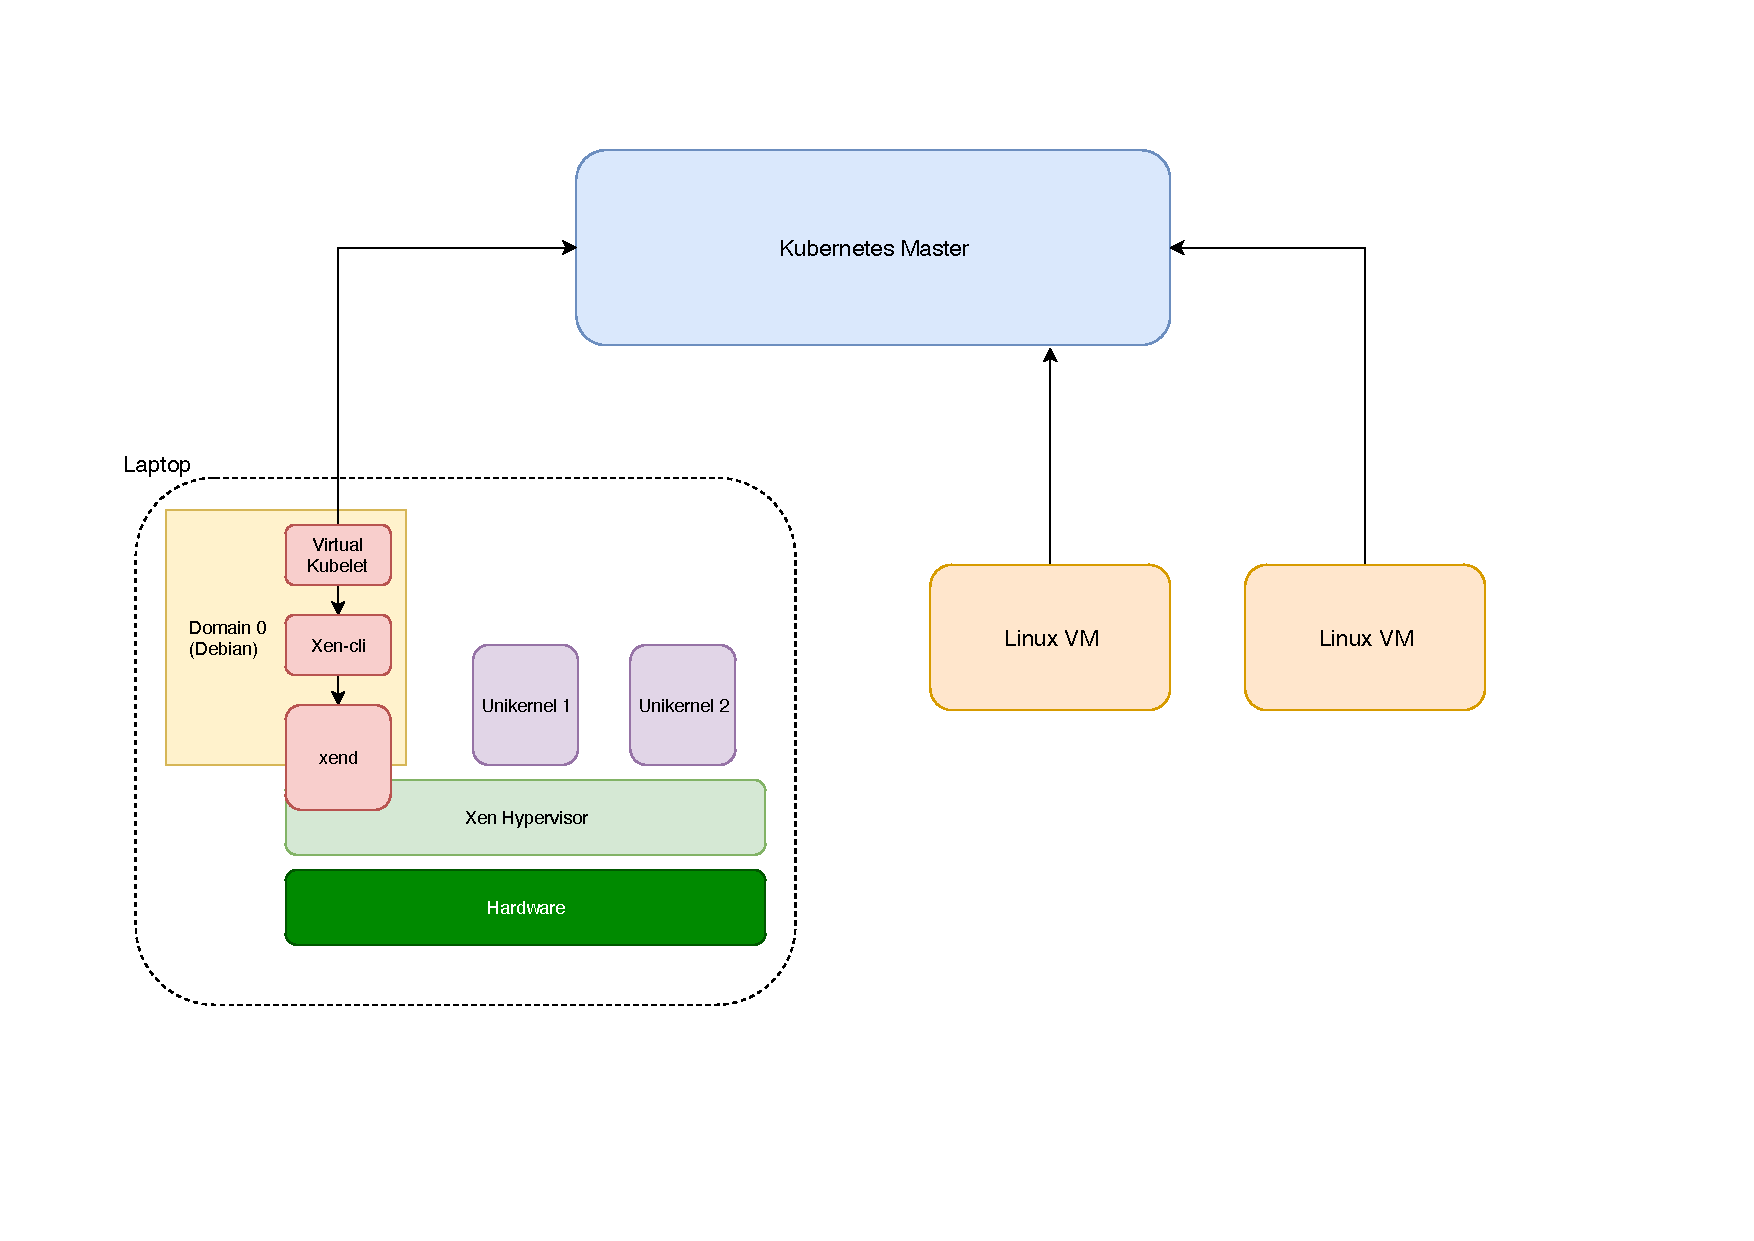
\includegraphics[width=1.2\textwidth]{figures/arch_new.pdf}
    \caption{ Kubernetes cluster with a only hypervisor enabled node for unikernel deployment} \label{fig:hypervisor}
  \end{figure}
%todo: kubeproxy
% todo: minios

\pagebreak